\chapter{Overview}

This section aims to briefly introduce the Raspberry Pi 3, give a clear overview of the physical testbed and the network topology.


\section{The Raspberry Pi 3 Cluster} \label{pi3cluster}

The Raspberry Pi is a series of small single-board computers developed in the United Kingdom by the Raspberry Pi Foundation to promote teaching of basic computer science in schools and in developing countries. The Raspberry Pi 3 Model B+ was released in 2018, and is the model used in this cluster.

\begin{table}[H]
    \centering
    \begin{tabular}{ |p{4cm}|p{2cm}|p{4cm}|p{2cm}|p{2cm}|  }
        \hline
        \multicolumn{5}{|c|}{\textbf{Raspberry Pi 3 Model B+ Specifications}} \\
        \hline
        \textbf{CPU} & \textbf{RAM} & \textbf{NICs} & \textbf{Storage} & \textbf{USB}\\
        \hline
        Broadcom BCM2837B0 \newline Cortex-A53 (ARMv8) 64-bit SoC \newline 1.4GHz, Quad-core &
        1 GB LPDDR2 SDRAM &
        Gigabit Ethernet over USB 2.0 \newline Dual IEEE 802.11ac WiFi, Bluetooth 4.2 &
        32GB Micro-SD &
        4 USB 2.0 ports\\
        \hline
    \end{tabular}
    \caption{The hardware specifications of Raspberry Pi 3 Model B+.}
\end{table}

The cluster consists of eight Raspberry Pi 3 Model B+ machines, all hooked up to a Zyxel switch. The switch provides interconnectivity, but also powers the machines through \gls{poe}.

\begin{figure}[H]
    \centering
    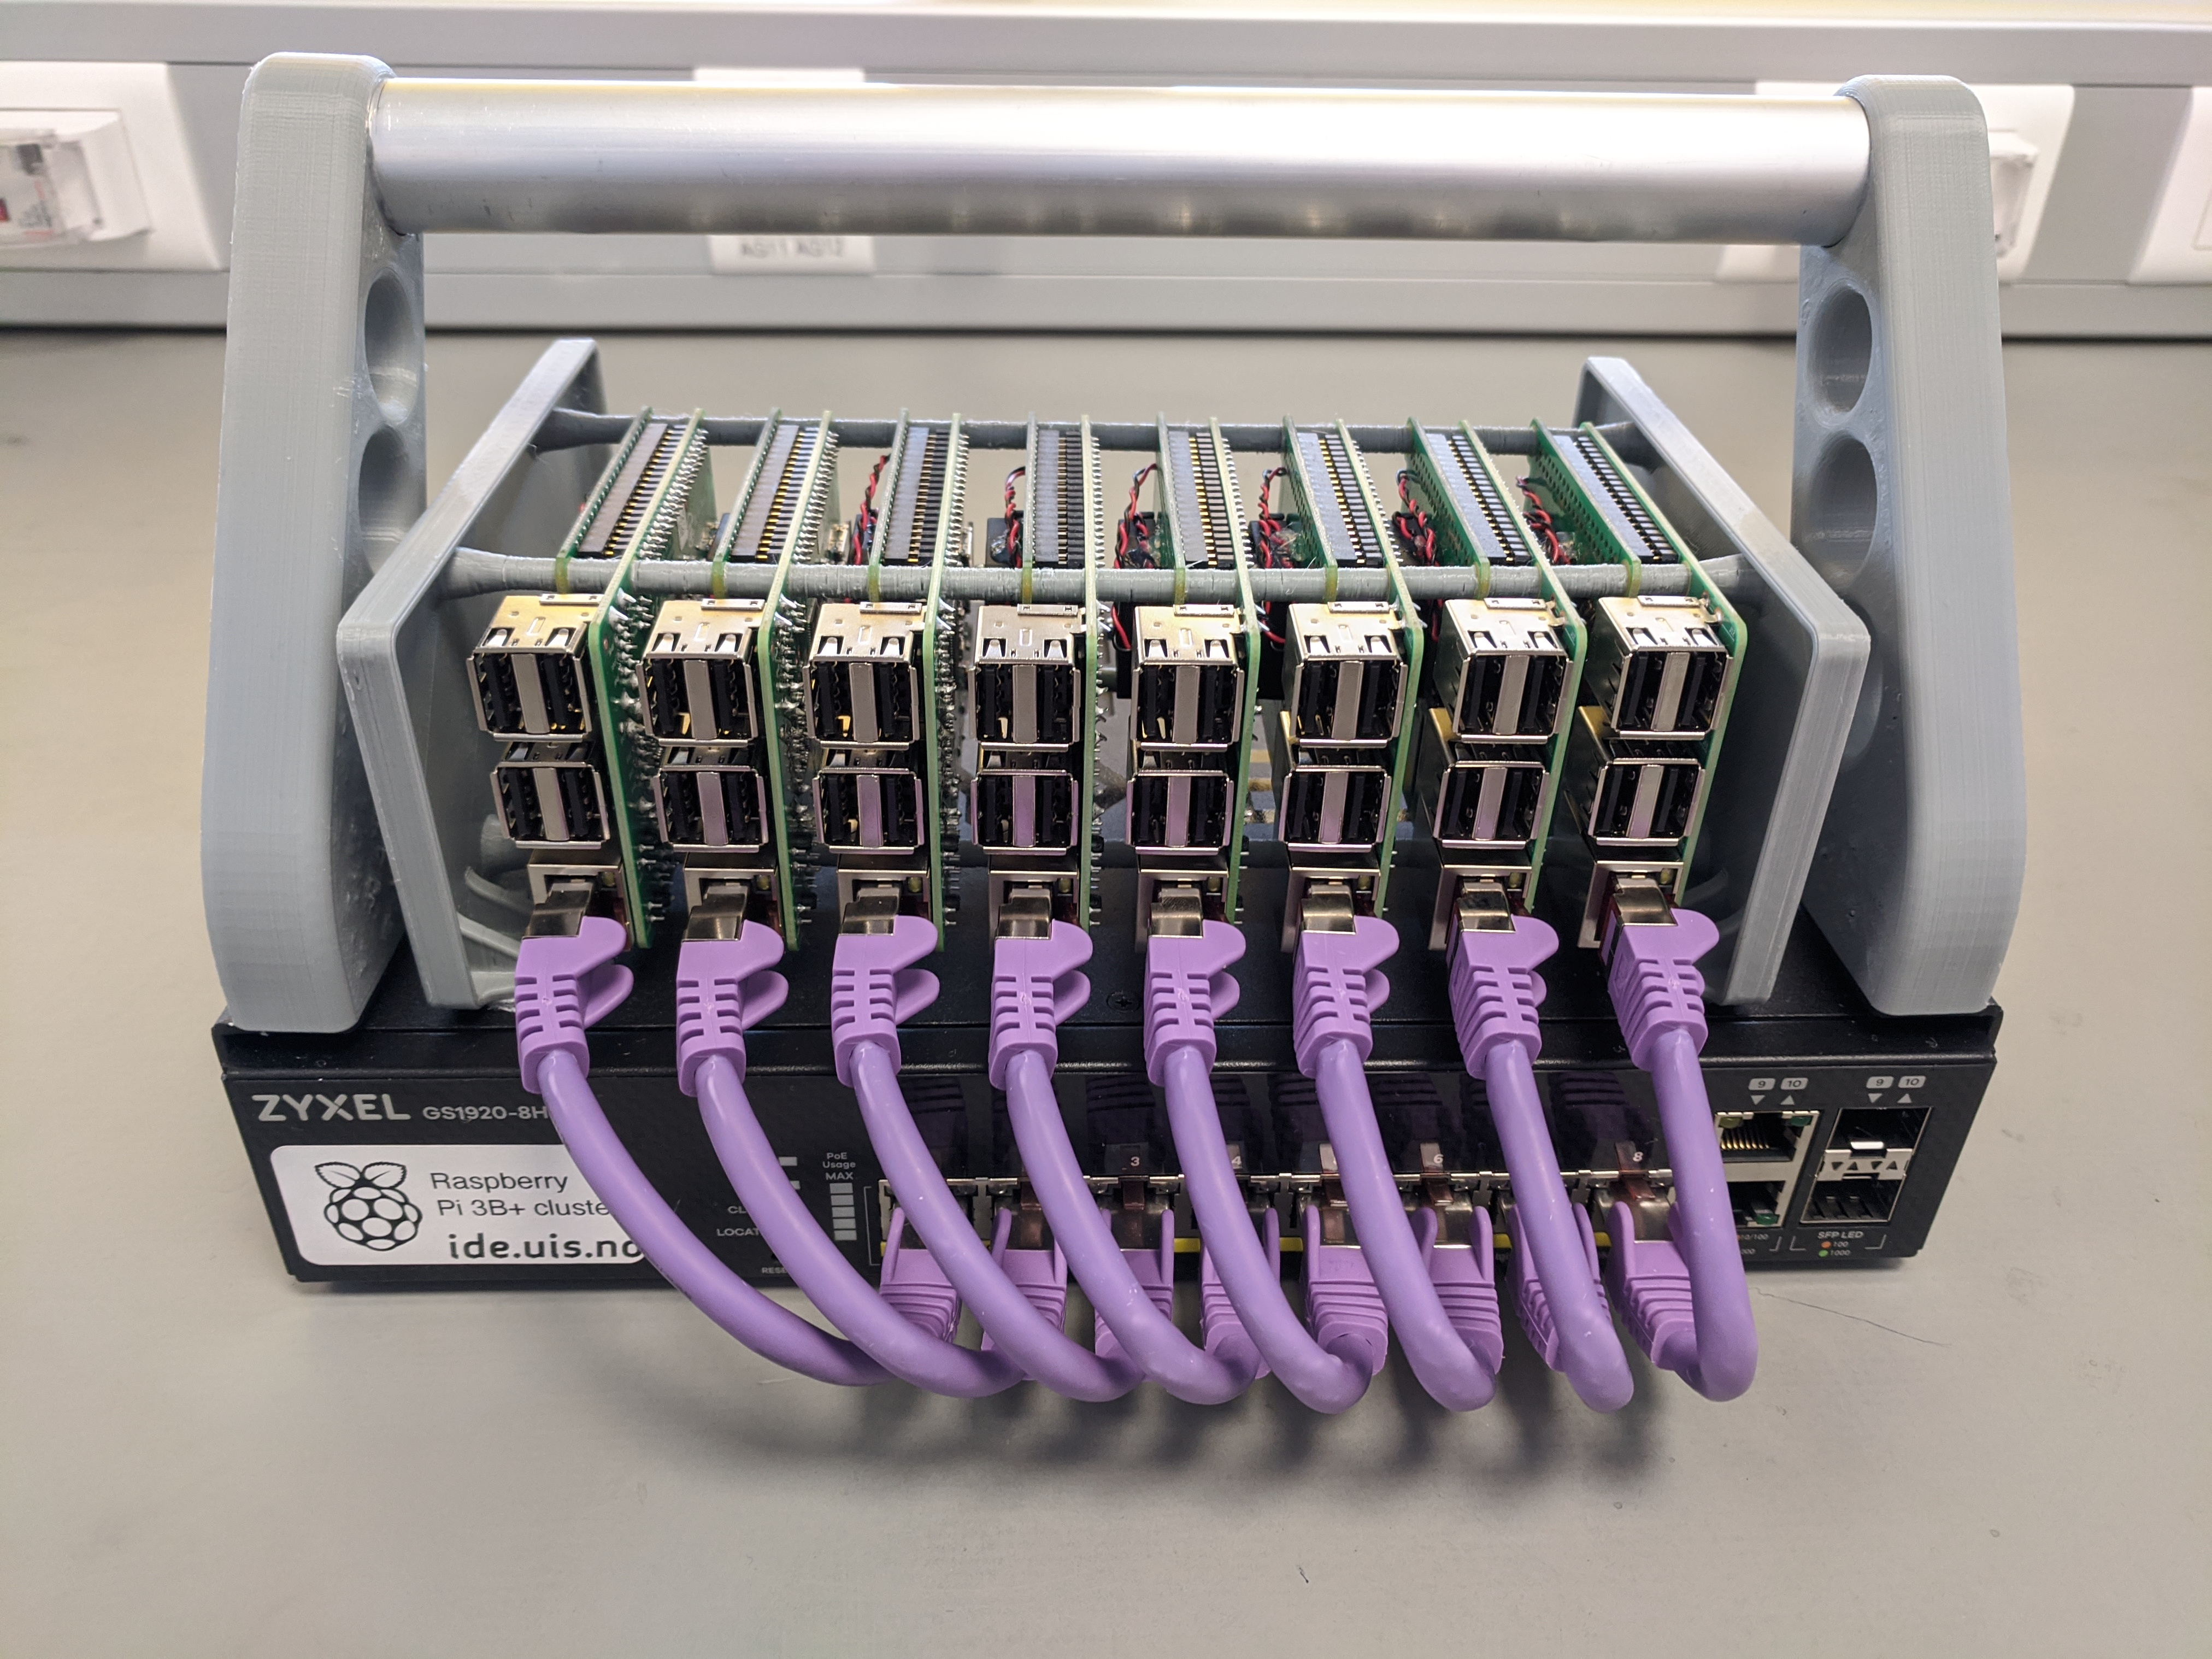
\includegraphics[width=0.6\linewidth]{pi3cluster}
    \captionsetup{width=0.6\linewidth}
    \caption{The Raspberry Pi 3B+ cluster all hooked to a Zyxel switch.}
    \label{fig:pi3cluster}
\end{figure}

\section{Network Topology} \label{topology}

The testbed consists of two networks; the \textit{controller} network in which all machines are connected directly, and the \textit{experimental} network separated by two subnets with a router in-between.

\begin{figure}[H]
    \centering
    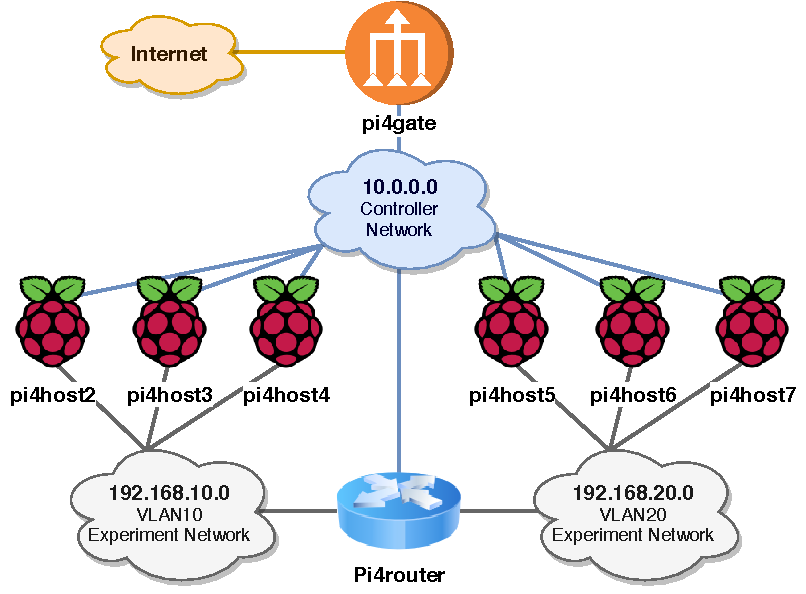
\includegraphics[width=0.8\linewidth]{network_topology}
    \captionsetup{width=0.8\linewidth}
    \caption{The logical network topology for the Raspberry Pi 3B+ cluster testbed.}
    \label{fig:network_topology}
\end{figure}

Since the entire testbed is connected to a single switch only, both \gls{vlan} and virtual interfaces have been used to achieve the desired network topology. In addition, one USB-to-ethernet adapter was necessary on the router in order to conduct network experimentation with TEACUP. The \gls{vlan} setup on the switch is explained in section \ref{zyxel} while the general network setup for every machine is explained in the remaining sections.

A summary table of the network setup for each machine follows.

\begin{table}[H]
    \centering
    \begin{tabular}{ |p{2cm}|p{6cm}|p{3cm}|  }
        \hline
        \multicolumn{3}{|c|}{\textbf{Summary Network Setup}} \\
        \hline
        \textbf{Hostname} & \textbf{IP address} & \textbf{OS}\\
        \hline
        pi3router & 10.0.1.1 --- eth0 \newline 172.16.10.1 --- eth0:10 (virtual) \newline 172.16.20.1 --- eth1 (USB-to-eth) & Raspbian Buster (Linux)\\
        \hline
        pi3host2 & 10.0.1.2 --- eth0 \newline 172.16.10.2 --- eth0:10 (virtual) & FreeBSD 12.1\\
        \hline
        pi3host3 & 10.0.1.3 --- eth0 \newline 172.16.10.3 --- eth0:10 (virtual) & FreeBSD 12.1\\
        \hline
        pi3host4 & 10.0.1.4 --- eth0 \newline 172.16.10.4 --- eth0:10 (virtual) & FreeBSD 12.1\\
        \hline
        pi3host5 & 10.0.1.5 --- eth0 \newline 172.16.20.5 --- eth0:20 (virtual) & FreeBSD 12.1\\
        \hline
        pi3host6 & 10.0.1.6 --- eth0 \newline 172.16.20.6 --- eth0:20 (virtual) & FreeBSD 12.1\\
        \hline
        pi3host7 & 10.0.1.7 --- eth0 \newline 172.16.20.7 --- eth0:20 (virtual) & FreeBSD 12.1\\
        \hline
        pi3gate & DHCP --- eth0 \newline 10.0.1.254 --- eth0:1 (virtual) & Raspbian Buster (Linux)\\
        \hline
    \end{tabular}
    \caption{The hostnames, IP addresses and OS for each Raspberry Pi 3B+ machine in the cluster.}
\end{table}

The table above lists the configured Raspberry Pi 3B+ machines in left to right order as seen from \ref{fig:pi3cluster}. That is, the left most machine is set up as the router, and the right most machine is set up as the gateway.